\begin{knitrout}
\definecolor{shadecolor}{rgb}{0.969, 0.969, 0.969}\color{fgcolor}\begin{figure}

{\centering 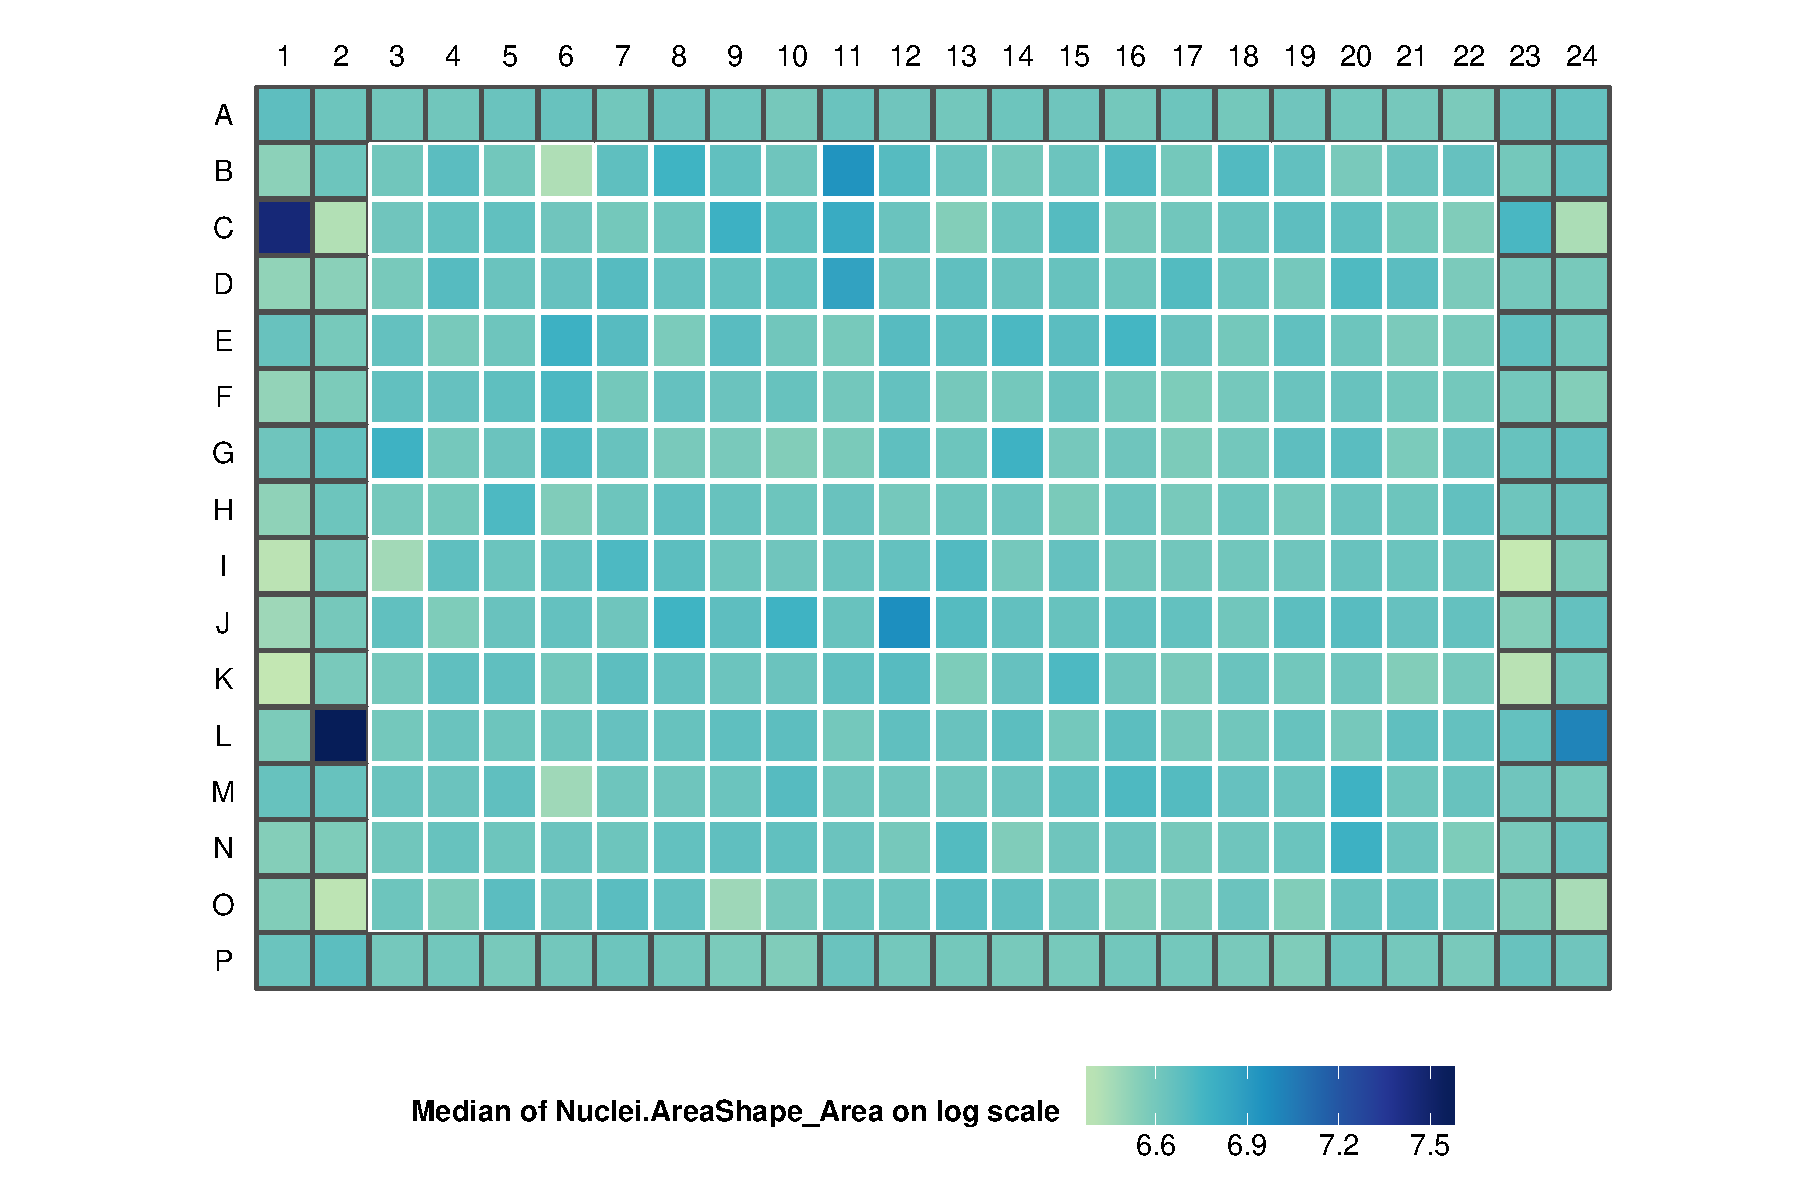
\includegraphics[width=.95\linewidth]{figures/R/heatmap-demo-scf-heatmap-1} 

}

\caption[An example heatmap plot as produced by \mintinline{text}{plateHeatmap}.]{Several visualization procedures are integrated with singelCellFeatures. In this example, the median of the feature Nuclei.AreaShape\_Area is shown on a logarithmic scale. Two parameters of \mintinline{text}{plateHeatmap} are functions so that the user can customize both, how data per well is summarized and on what scale colors are determined. The plate is J101-2C (wells C1, L2, C23 and L24 contain cell killer \gls{kif11} \gls{sirna}).}\label{fig:scf-heatmap}
\end{figure}


\end{knitrout}
